\PassOptionsToPackage{unicode}{hyperref}
\documentclass[aspectratio=1610, 11pt]{beamer}

\usepackage{amsmath}
\usepackage{amssymb}
\usetheme{tudo}

\title{Datenstrukturen, Algorithmen und Programmierung~2}
\author[A.~Coja-Oghlan]{Amin Coja-Oghlan}
\institute[DAP2]{Lehrstuhl Informatik 2\\Fakult\"at f\"ur Informatik}

\newcommand\dist{\mathrm{dist}}
\renewcommand{\vec}[1]{\boldsymbol{#1}}
\newcommand\NULL{{\tt NULL}}
\newcommand\dd{\mathrm d}
\newcommand\eul{\mathrm e}
\newcommand\cA{\mathcal A}
\newcommand\cB{\mathcal B}
\newcommand\cC{\mathcal C}
\newcommand\cD{\mathcal D}
\newcommand\cE{\mathcal E}
\newcommand\cF{\mathcal F}
\newcommand\cG{\mathcal G}
\newcommand\cH{\mathcal H}
\newcommand\cI{\mathcal I}
\newcommand\cJ{\mathcal J}
\newcommand\cK{\mathcal K}
\newcommand\cL{\mathcal L}
\newcommand\cM{\mathcal M}
\newcommand\cN{\mathcal N}
\newcommand\cO{\mathcal O}
\newcommand\cP{\mathcal P}
\newcommand\cQ{\mathcal Q}
\newcommand\cR{\mathcal R}
\newcommand\cS{\mathcal S}
\newcommand\cT{\mathcal T}
\newcommand\cU{\mathcal U}
\newcommand\cV{\mathcal V}
\newcommand\cW{\mathcal W}
\newcommand\cX{\mathcal X}
\newcommand\cY{\mathcal Y}
\newcommand\cZ{\mathcal Z}
\newcommand\fA{\mathfrak A}
\newcommand\fB{\mathfrak B}
\newcommand\fC{\mathfrak C}
\newcommand\fD{\mathfrak D}
\newcommand\fE{\mathfrak E}
\newcommand\fF{\mathfrak F}
\newcommand\fG{\mathfrak G}
\newcommand\fH{\mathfrak H}
\newcommand\fI{\mathfrak I}
\newcommand\fJ{\mathfrak J}
\newcommand\fK{\mathfrak K}
\newcommand\fL{\mathfrak L}
\newcommand\fM{\mathfrak M}
\newcommand\fN{\mathfrak N}
\newcommand\fO{\mathfrak O}
\newcommand\fP{\mathfrak P}
\newcommand\fQ{\mathfrak Q}
\newcommand\fR{\mathfrak R}
\newcommand\fS{\mathfrak S}
\newcommand\fT{\mathfrak T}
\newcommand\fU{\mathfrak U}
\newcommand\fV{\mathfrak V}
\newcommand\fW{\mathfrak W}
\newcommand\fX{\mathfrak X}
\newcommand\fY{\mathfrak Y}
\newcommand\fZ{\mathfrak Z}
\newcommand\fa{\mathfrak a}
\newcommand\fb{\mathfrak b}
\newcommand\fc{\mathfrak c}
\newcommand\fd{\mathfrak d}
\newcommand\fe{\mathfrak e}
\newcommand\ff{\mathfrak f}
\newcommand\fg{\mathfrak g}
\newcommand\fh{\mathfrak h}
%\newcommand\fi{\mathfrak i}
\newcommand\fj{\mathfrak j}
\newcommand\fk{\mathfrak k}
\newcommand\fl{\mathfrak l}
\newcommand\fm{\mathfrak m}
\newcommand\fn{\mathfrak n}
\newcommand\fo{\mathfrak o}
\newcommand\fp{\mathfrak p}
\newcommand\fq{\mathfrak q}
\newcommand\fr{\mathfrak r}
\newcommand\fs{\mathfrak s}
\newcommand\ft{\mathfrak t}
\newcommand\fu{\mathfrak u}
\newcommand\fv{\mathfrak v}
\newcommand\fw{\mathfrak w}
\newcommand\fx{\mathfrak x}
\newcommand\fy{\mathfrak y}
\newcommand\fz{\mathfrak z}
\newcommand\vA{\vec A}
\newcommand\vB{\vec B}
\newcommand\vC{\vec C}
\newcommand\vD{\vec D}
\newcommand\vE{\vec E}
\newcommand\vF{\vec F}
\newcommand\vG{\vec G}
\newcommand\vH{\vec H}
\newcommand\vI{\vec I}
\newcommand\vJ{\vec J}
\newcommand\vK{\vec K}
\newcommand\vL{\vec L}
\newcommand\vM{\vec M}
\newcommand\vN{\vec N}
\newcommand\vO{\vec O}
\newcommand\vP{\vec P}
\newcommand\vQ{\vec Q}
\newcommand\vR{\vec R}
\newcommand\vS{\vec S}
\newcommand\vT{\vec T}
\newcommand\vU{\vec U}
\newcommand\vV{\vec V}
\newcommand\vW{\vec W}
\newcommand\vX{\vec X}
\newcommand\vY{\vec Y}
\newcommand\vZ{\vec Z}
\newcommand\va{\vec a}
\newcommand\vb{\vec b}
\newcommand\vc{\vec c}
\newcommand\vd{\vec d}
\newcommand\ve{\vec e}
\newcommand\vf{\vec f}
\newcommand\vg{\vec g}
\newcommand\vh{\vec h}
\newcommand\vi{\vec i}
\newcommand\vj{\vec j}
\newcommand\vk{\vec k}
\newcommand\vl{\vec l}
\newcommand\vm{\vec m}
\newcommand\vn{\vec n}
\newcommand\vo{\vec o}
\newcommand\vp{\vec p}
\newcommand\vq{\vec q}
\newcommand\vr{\vec r}
\newcommand\vs{\vec s}
\newcommand\vt{\vec t}
\newcommand\vu{\vec u}
\renewcommand\vv{\vec v}
\newcommand\vw{\vec w}
\newcommand\vx{\vec x}
\newcommand\vy{\vec y}
\newcommand\vz{\vec z}
\renewcommand\AA{\mathbb A}
\newcommand\NN{\mathbb N}
\newcommand\ZZ{\mathbb Z}
\newcommand\PP{\mathbb P}
\newcommand\QQ{\mathbb Q}
\newcommand\RR{\mathbb R}
\newcommand\RRpos{\mathbb R_{\geq0}}
\newcommand\QQpos{\mathbb Q_{\geq0}}
\renewcommand\SS{\mathbb S}
\newcommand\CC{\mathbb C}
\newcommand{\ord}{\mathrm{ord}}
\newcommand{\id}{\mathrm{id}}
\newcommand{\pr}{\mathrm{P}}
\newcommand{\Vol}{\mathrm{vol}}
\newcommand\norm[1]{\left\|{#1}\right\|} 
\newcommand\sign{\mathrm{sign}}
\newcommand{\eps}{\varepsilon}
\newcommand{\abs}[1]{\left|#1\right|}
\newcommand\bc[1]{\left({#1}\right)} 
\newcommand\cbc[1]{\left\{{#1}\right\}} 
\newcommand\bcfr[2]{\bc{\frac{#1}{#2}}} 
\newcommand{\bck}[1]{\left\langle{#1}\right\rangle} 
\newcommand\brk[1]{\left\lbrack{#1}\right\rbrack} 
\newcommand\scal[2]{\bck{{#1},{#2}}} 
\newcommand{\vecone}{\mathbb{1}}
\newcommand{\tensor}{\otimes}
\newcommand{\diag}{\mathrm{diag}}
\newcommand{\ggt}{\mathrm{ggT}}
\newcommand{\kgv}{\mathrm{kgV}}
\newcommand{\trans}{\top}
\newcommand{\Karonski}{Karo\'nski}
\newcommand{\Erdos}{Erd\H{o}s}
\newcommand{\Renyi}{R\'enyi}
\newcommand{\Lovasz}{Lov\'asz}
\newcommand{\Juhasz}{Juh\'asz}
\newcommand{\Bollobas}{Bollob\'as}
\newcommand{\Furedi}{F\"uredi}
\newcommand{\Komlos}{Koml\'os}
\newcommand{\Luczak}{\L uczak}
\newcommand{\Kucera}{Ku\v{c}era}
\newcommand{\Szemeredi}{Szemer\'edi}

\newcommand{\mytitle}{Bin\"are Suchb\"aume}

\begin{document}

\frame[plain]{\titlepage}

\begin{frame}\frametitle{\mytitle}
	\begin{exampleblock}{Worum geht es?}
		\begin{itemize}
			\item ein bin\"arer Suchbaum ist eine Datenstruktur zur Speicherung von Objekten, die durch einen Schl\"ussel gekennzeichnet sind
			\item die Schl\"ussel sind total geordnet
			\item wir nehmen an, da\ss\ alle Schl\"ussel verschieden sind
			\item \alert{Operationen:} {\tt Insert}, {\tt Delete}, {\tt Search}, {\tt Minimum}, {\tt Maximum}, {\tt Predecessor}, {\tt Successor}
			\item die Laufzeit jeder Operation ist $O(\mbox{H\"ohe des Baums})$
		\end{itemize}
	\end{exampleblock}
\end{frame}

\begin{frame}\frametitle{\mytitle}
	\hfill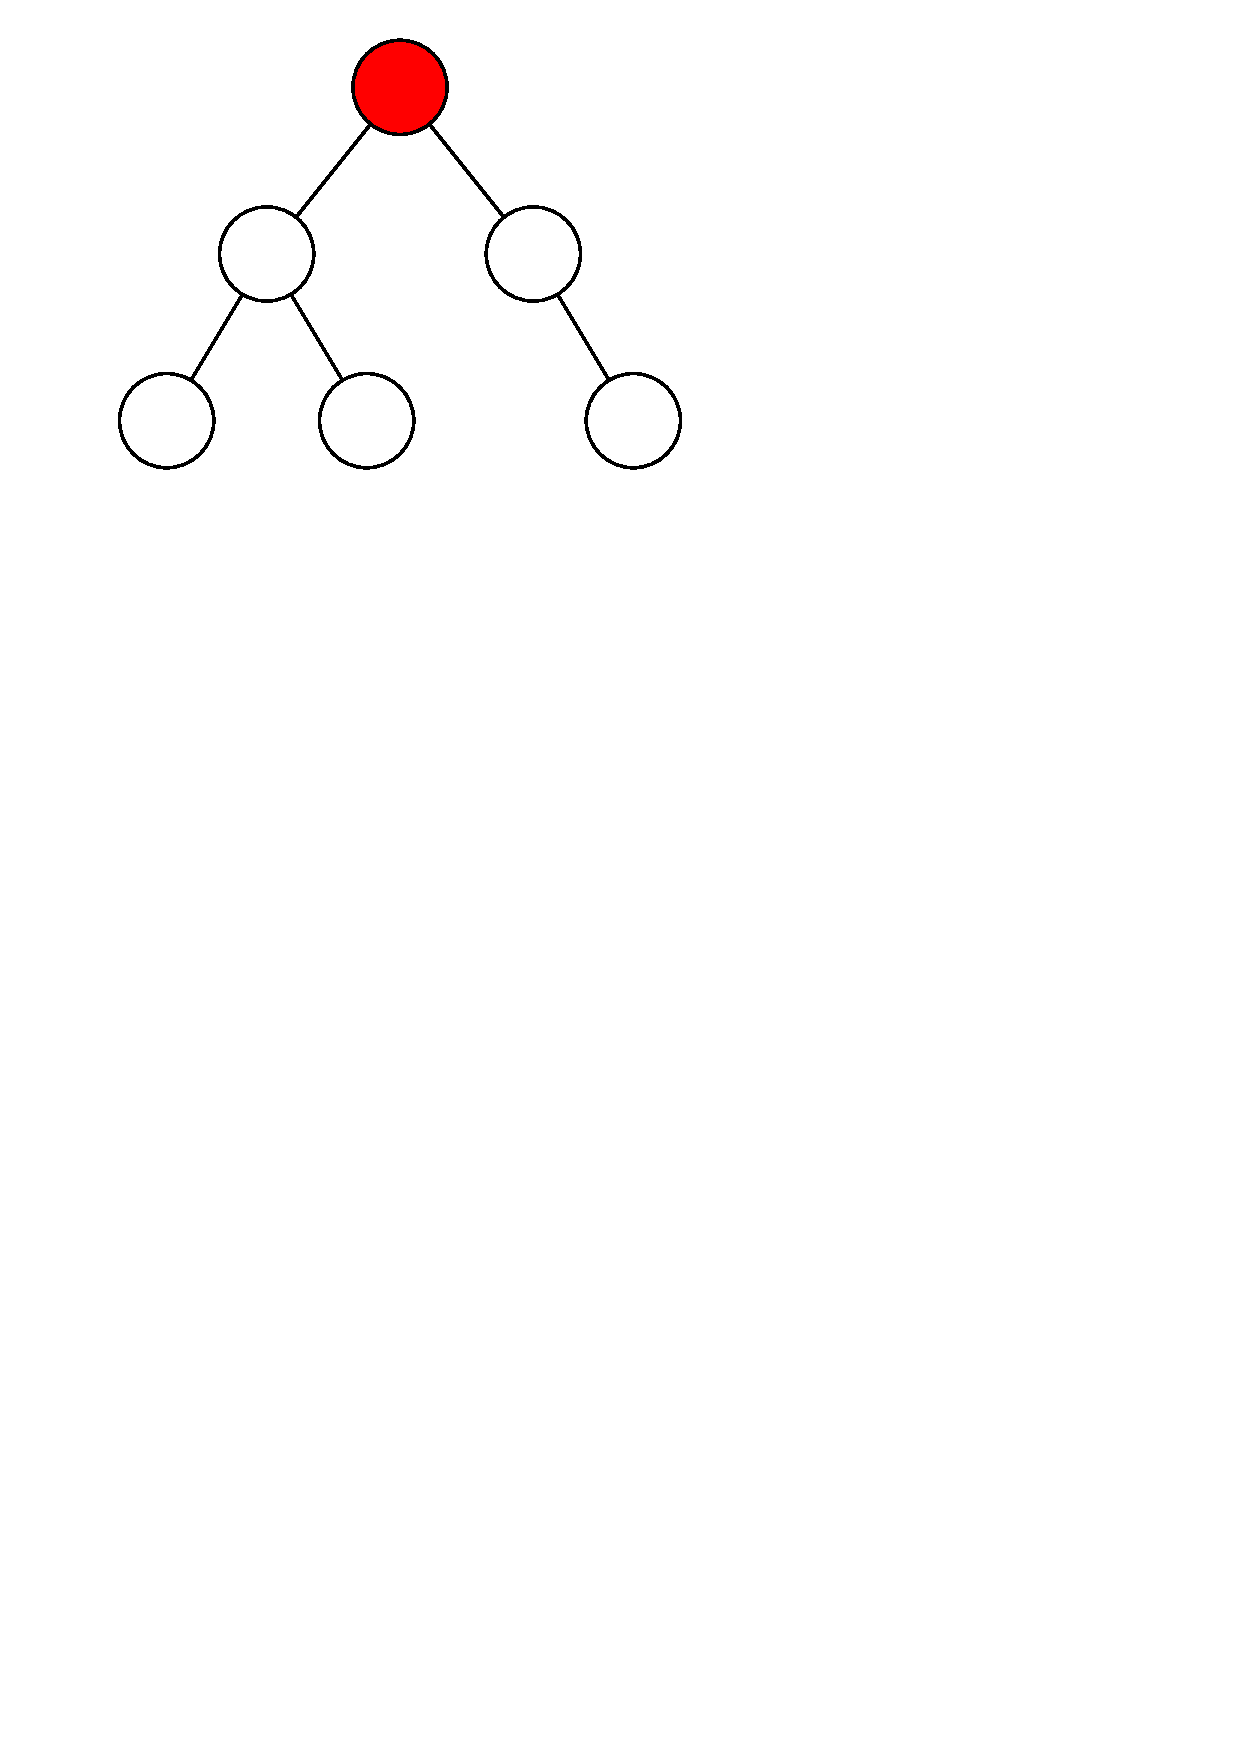
\includegraphics[height=20mm]{./images/binary_tree.pdf}
	\begin{exampleblock}{Bin\"arb\"aume}
		\begin{itemize}
			\item ein \alert{Bin\"arbaum} ist ein gewurzelter Baum, d.h.\ ein Baum $T$ mit einer ausgezeichneten Wurzel $r\in V(T)$
			\item die Wurzel hat Grad $d_T(r)\leq2$
			\item jeder andere Knoten $v\in V(T)\setminus\{r\}$ hat Grad $\leq3$
			\item die \alert{Kinder} eines Knotens $v$ sind die Nachbarn $w\in\partial v$, die nicht auf dem k\"urzsten Pfad von $v$ nach $r$ liegen; jeder Knoten hat also h\"ochstens zwei Kinder
			\item der \alert{Elternknoten} von $v$ ist der Nachbar auf dem k\"urzesten Pfad zu $r$, bzw.\ $\emptyset$ falls $v=r$
		\end{itemize}
	\end{exampleblock}
\end{frame}

\begin{frame}\frametitle{\mytitle}
	\hfill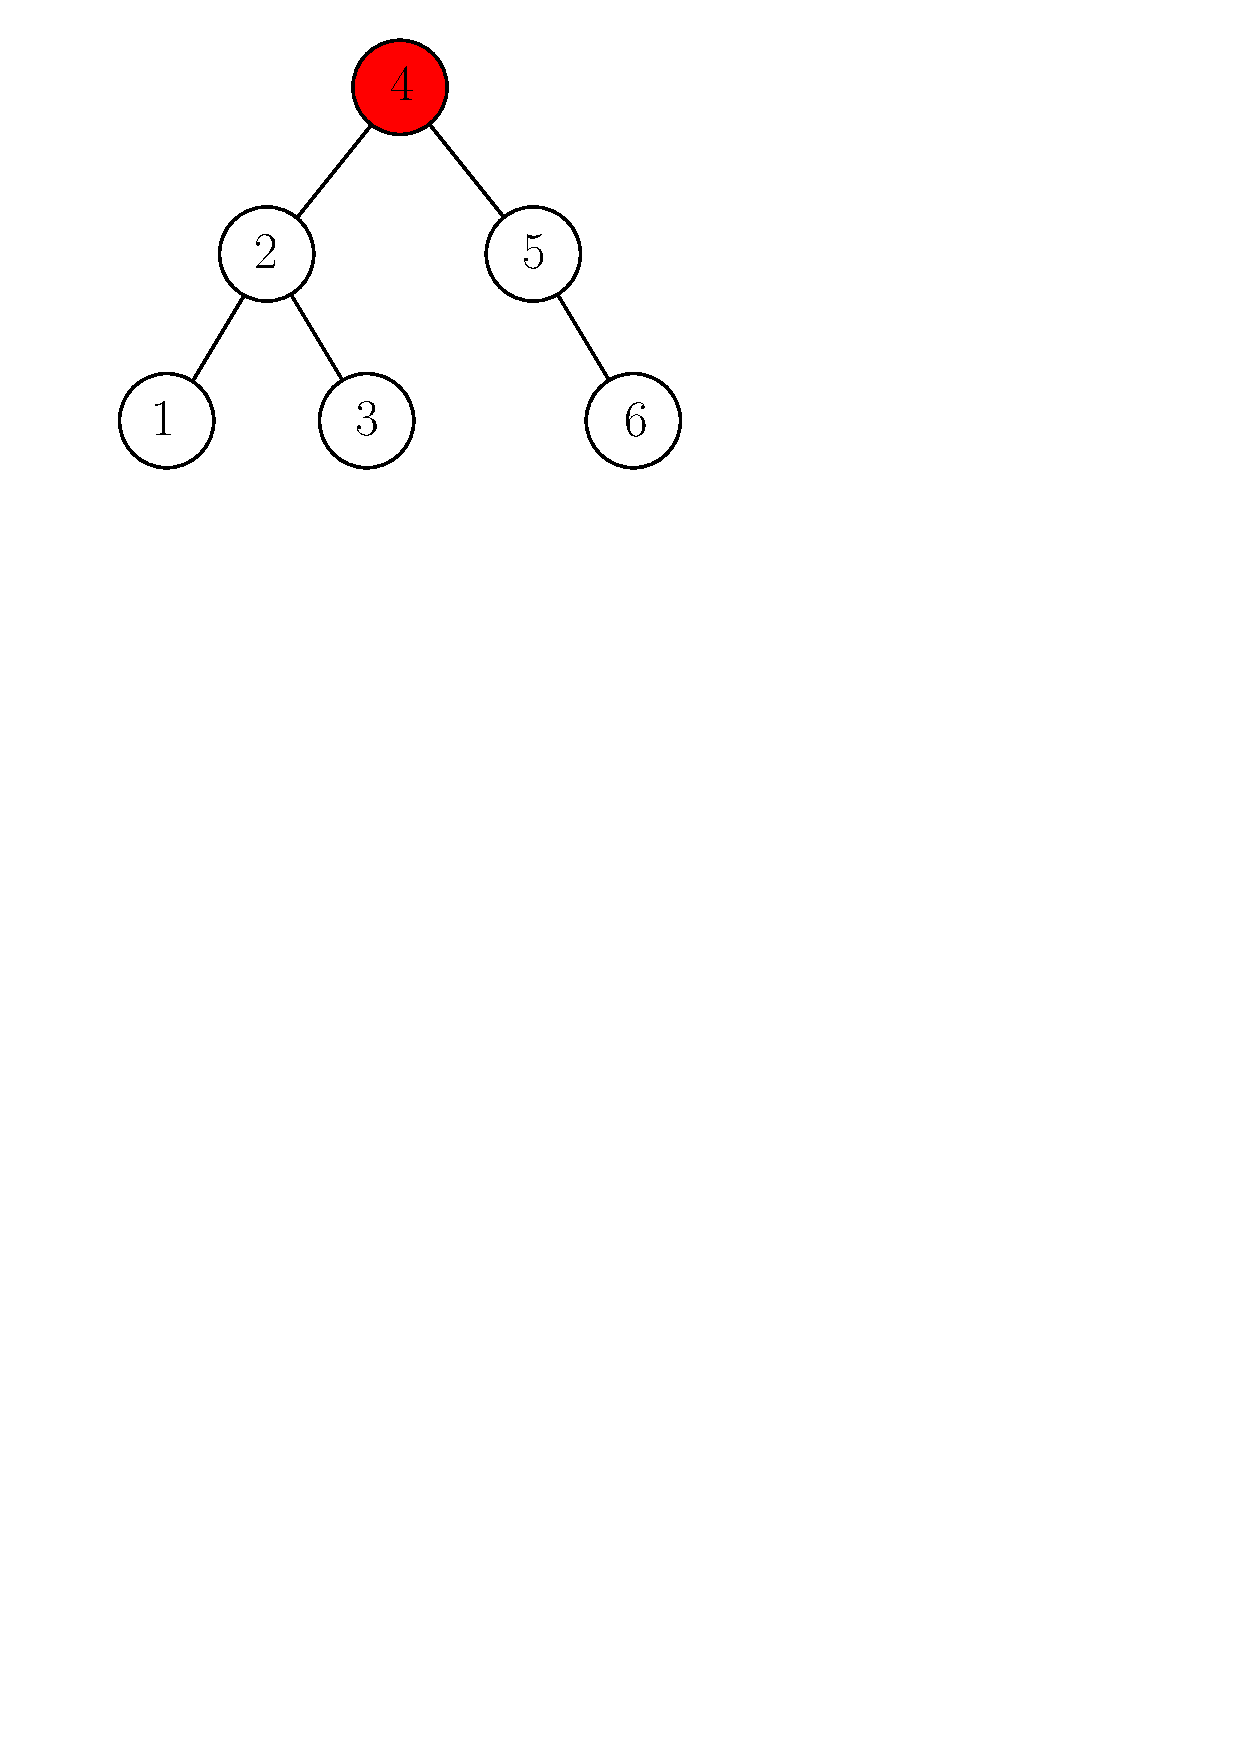
\includegraphics[height=30mm]{./images/binary_searchtree.pdf}
	\begin{overprint}
		\onslide<1>
		\begin{exampleblock}{Suchb\"aume}
			\begin{itemize}
				\item die Knoten tragen vergleichbare \alert{Schl\"ussel} $s(v)$
				\item sei $v$ ein Knoten
				\item dann hat $v$ h\"ochstens ein Kind $x$ mit $s(x)<s(v)$
				\item ferner hat $v$ h\"ochstens ein Kind $y$ mit $s(y)>s(v)$
				\item wir nennen $x$ das \alert{linke Kind} von $v$ und $y$ das \alert{rechte Kind}
			\end{itemize}
		\end{exampleblock}
		\onslide<2>
		\begin{exampleblock}{Suchb\"aumeigenschaft}
			\begin{itemize}
				\item der Knoten $x$ und seine Kinder bilden den \alert{linken Unterbaum} von $v$
				\item der Knoten $y$ und seine Kinder bilden den \alert{rechten Unterbaum} von $v$
				\item \alert{Suchbaumeigenschaft:} f\"ur alle Knoten $u$ im linken Unterbaum von $v$ gilt $s(u)<s(v)$; f\"ur alle Knoten $w$ im rechten Unterbaum von $v$ gilt $s(v)<s(w)$
			\end{itemize}
		\end{exampleblock}
		\onslide<3>
		\begin{exampleblock}{Implementation}
			\begin{itemize}
				\item jeder Knoten des Suchbaums enth\"alt den Schl\"ussel und ggf.\ einen Zeiger auf das Objekt, das dieser Knoten repr\"asentiert
				\item jeder Knoten enth\"alt einen Zeiger auf seinen Elternknoten (evtl. $\emptyset$)
				\item jeder Knoten enth\"alt einen Zeiger auf das linke und einen auf das rechte Kind (ggf.\ $\emptyset$)
			\end{itemize}
		\end{exampleblock}
	\end{overprint}
\end{frame}

\begin{frame}\frametitle{\mytitle}
	\hfill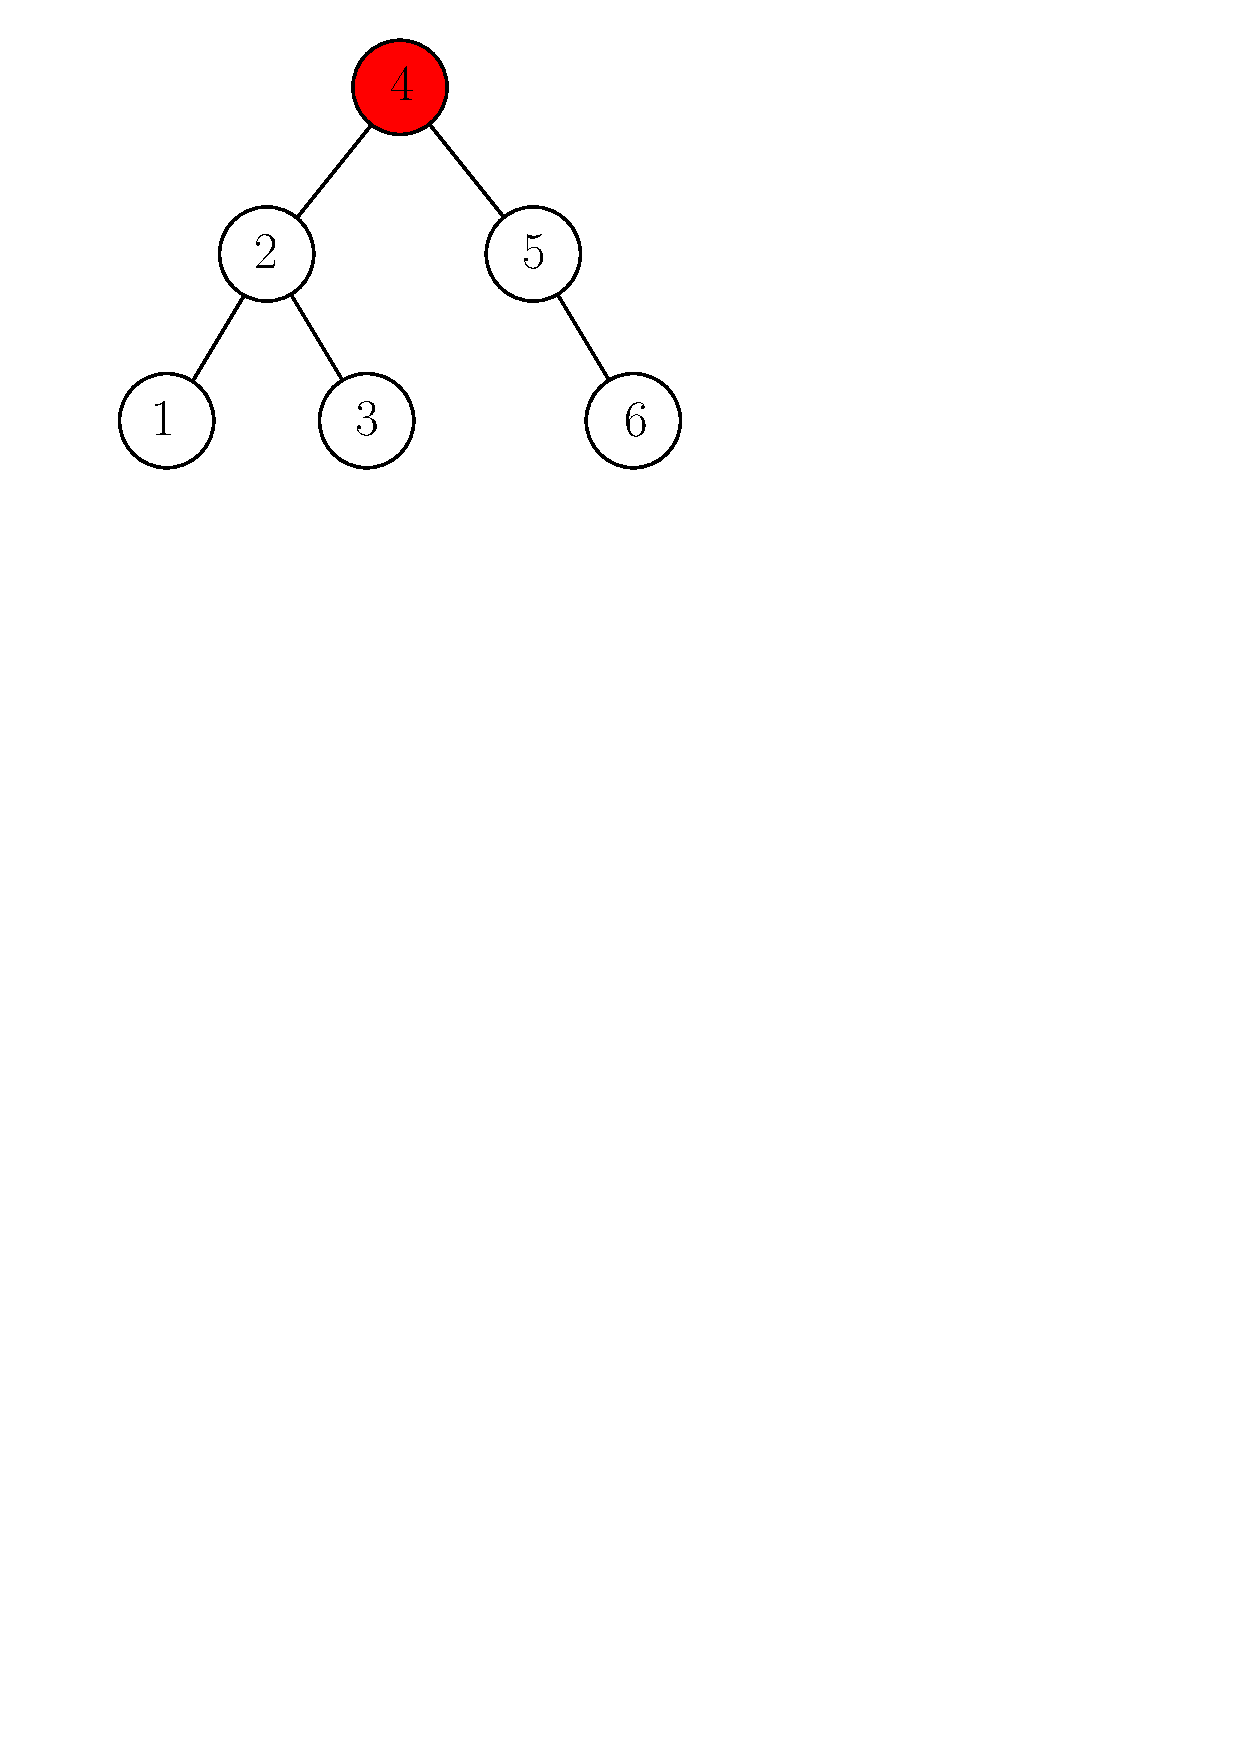
\includegraphics[height=30mm]{./images/binary_searchtree.pdf}
	\begin{overprint}
		\onslide<1>
		\begin{exampleblock}{Geordnete Ausgabe}
			\begin{itemize}
				\item wir k\"onnen die Elemente des Suchbaums ausgeben, indem wir von der Wurzel aus den Baum in Tiefensuchordnung durchlaufen
				\item dabei wird immer \alert{zuerst} das linke Kind aufgesucht, wenn eines existiert
			\end{itemize}
		\end{exampleblock}
		\onslide<2>
		\begin{exampleblock}{Minimum finden}
			\begin{itemize}
				\item um das Element mit minimalem Schl\"ussel zu finden, folgen wir von der Wurzel aus stets dem Zeiger auf das linke Kind
				\item der erste Knoten, dessen linkes Kind $\emptyset$ ist, ist das Minimum
			\end{itemize}
		\end{exampleblock}
		\onslide<3>
		\begin{exampleblock}{Maximum finden}
			\begin{itemize}
				\item um das Element mit maximalem Schl\"ussel zu finden, folgen wir von der Wurzel aus stets dem Zeiger auf das rechte Kind
				\item der erste Knoten, dessen rechtes Kind $\emptyset$ ist, ist das Maximum
			\end{itemize}
		\end{exampleblock}
		\onslide<4>
		\begin{exampleblock}{Element mit einem gegebenem Schl\"ussel suchen}
			\begin{itemize}
				\item die Operation {\tt Search} erh\"alt als Eingabe einen Schl\"ussel $\sigma$ und sucht das Element mit diesem Schl\"ussel
				\item von der Wurzel $v=r$ aus wiederhole folgendes Verfahren
			\end{itemize}
		\end{exampleblock}
		\onslide<5>
		\begin{exampleblock}{Element mit einem gegebenem Schl\"ussel suchen}
			\begin{itemize}
				\item falls $s(v)=\sigma$, gib $v$ aus
				\item falls $s(v)>\sigma$, setze $v$ auf das linke Kind $u$ von $v$; falls $u=\emptyset$, gib ``nicht vorhanden'' aus
				\item falls $s(v)<\sigma$, setze $v$ auf das rechte Kind $w$ von $v$; falls $w=\emptyset$, gib ``nicht vorhanden'' aus
			\end{itemize}
		\end{exampleblock}
		\onslide<6>
		\begin{exampleblock}{{\tt Successor}: gegeben $v$ finde $z$ mit minimalem $s(z)>s(v)$}
			\begin{itemize}
				\item falls $v$ ein rechtes Kind $w$ hat, finde das Minimum im rechten Teilbaum
				\item sonst setze $w$ auf den Elternknoten von $v$
				\item solange $w\neq\emptyset$ und $v$ das rechte Kind von $w$ ist, setze $v=w$ und $w=$Elternknoten von $v$
				\item gib schlie\ss lich $w$ aus
			\end{itemize}
		\end{exampleblock}
		\onslide<7>
		\begin{exampleblock}{{\tt Predecessor}: gegeben $v$ finde $z$ mit maximalem $s(z)<s(v)$}
			\begin{itemize}
				\item falls $v$ ein linkes Kind $w$ hat, finde das Maximum im linken Teilbaum
				\item sonst setze $w$ auf den Elternknoten von $v$
				\item solange $w\neq\emptyset$ und $v$ das linke Kind von $w$ ist, setze $v=w$ und $w=$Elternknoten von $v$
				\item gib schlie\ss lich $w$ aus
			\end{itemize}
		\end{exampleblock}
		\onslide<8>
		\begin{exampleblock}{Laufzeiten}
			\begin{itemize}
				\item die \alert{H\"ohe} $H(T)$ von $T$ ist der maximale Abstand von $r$ zu einem Blatt
				\item alle vorgenannten Operationen haben Laufzeit $O(H(T))$
			\end{itemize}
		\end{exampleblock}
	\end{overprint}
\end{frame}

\begin{frame}\frametitle{\mytitle}
	\hfill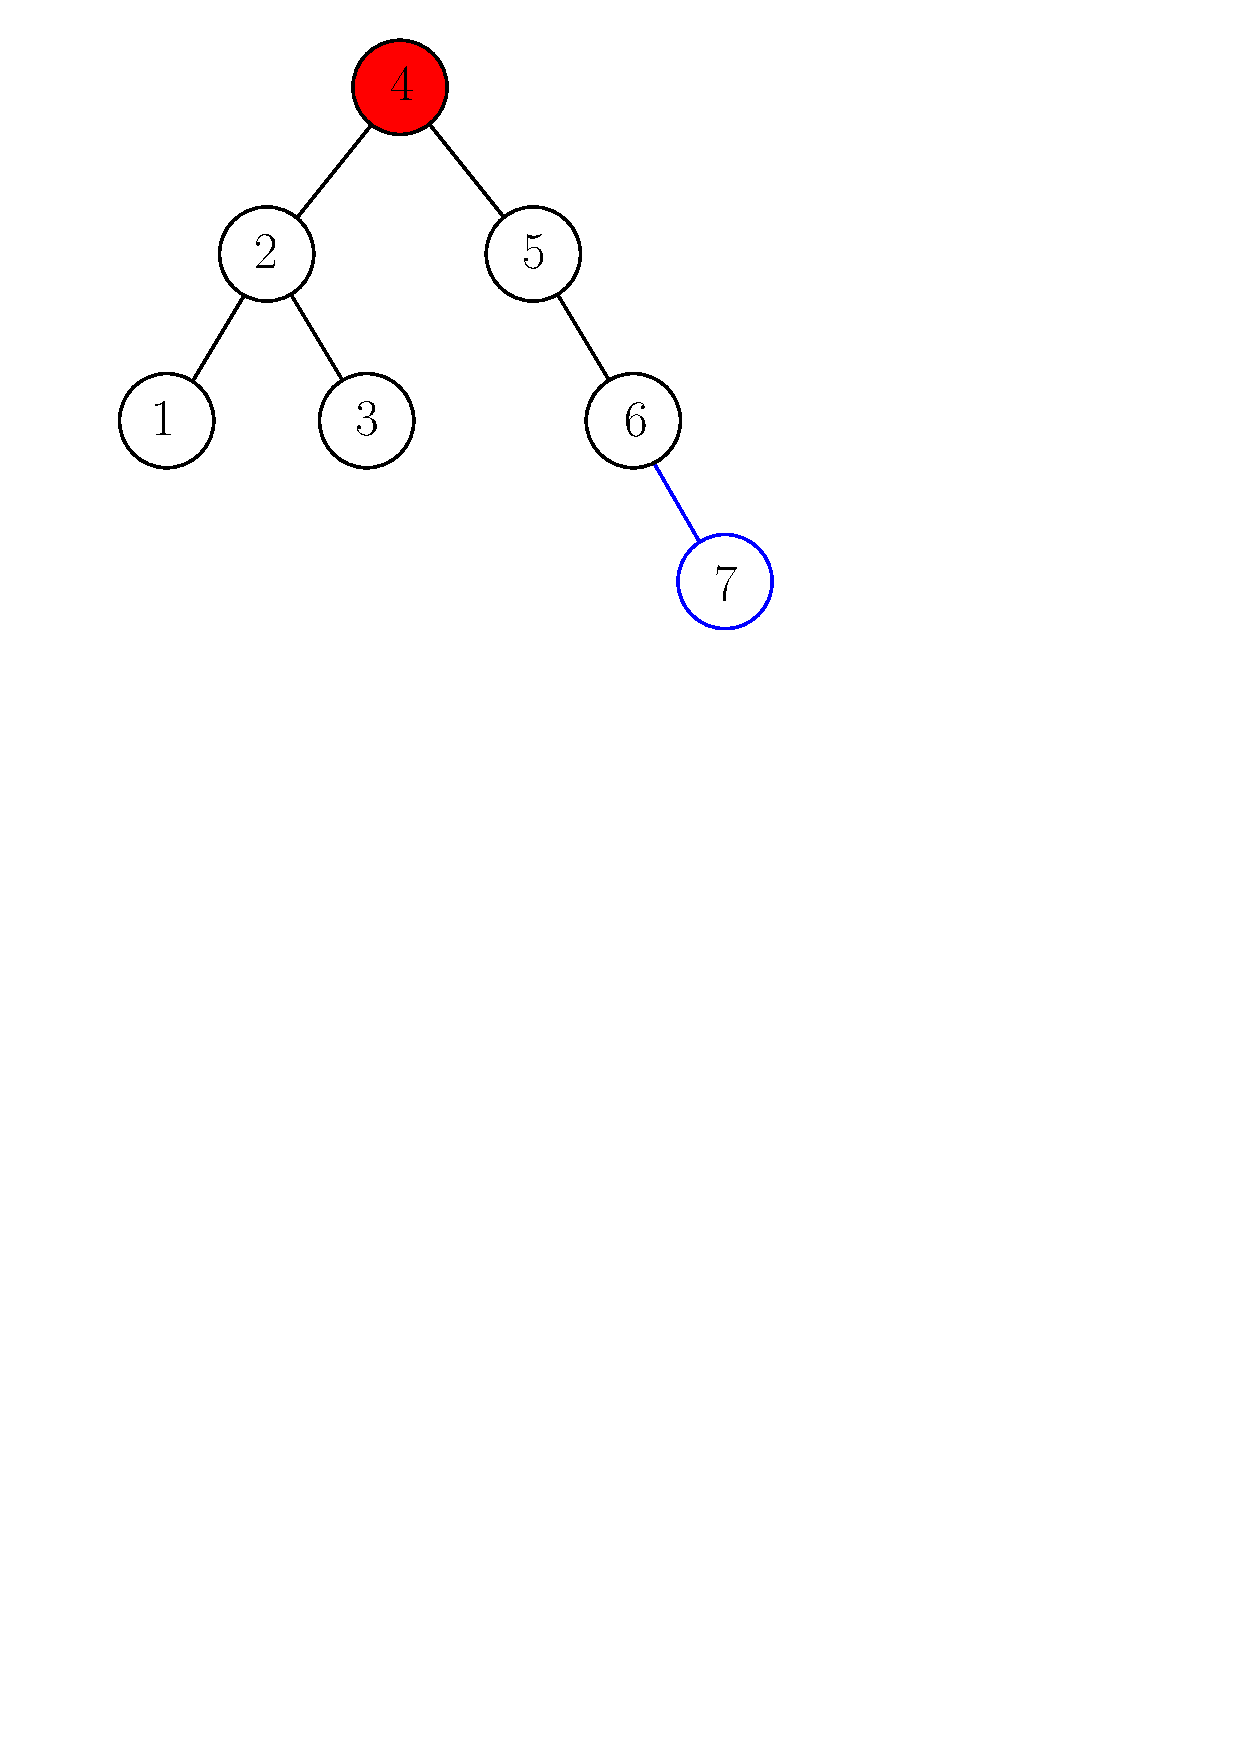
\includegraphics[height=30mm]{./images/binary_searchtree2.pdf}
	\begin{overprint}
		\onslide<1>
		\begin{exampleblock}{Einf\"ugen}
			\begin{itemize}
				\item um ein Element $e$ mit einem gegeben Schl\"ussel $s(e)$ einzuf\"ugen, gehen wir so vor, als w\"urden wir den Baum nach $e$ durchsuchen
				\item weil wir annehmen, da\ss\ $s(e)$ nicht im Baum vorkommt, finden wir dabei schlie\ss lich einen $\emptyset$-Zeiger
				\item diesen ersetzen wir durch das neue Element
			\end{itemize}
		\end{exampleblock}
	\end{overprint}
\end{frame}

\begin{frame}\frametitle{\mytitle}
	\begin{overprint}
		\onslide<1>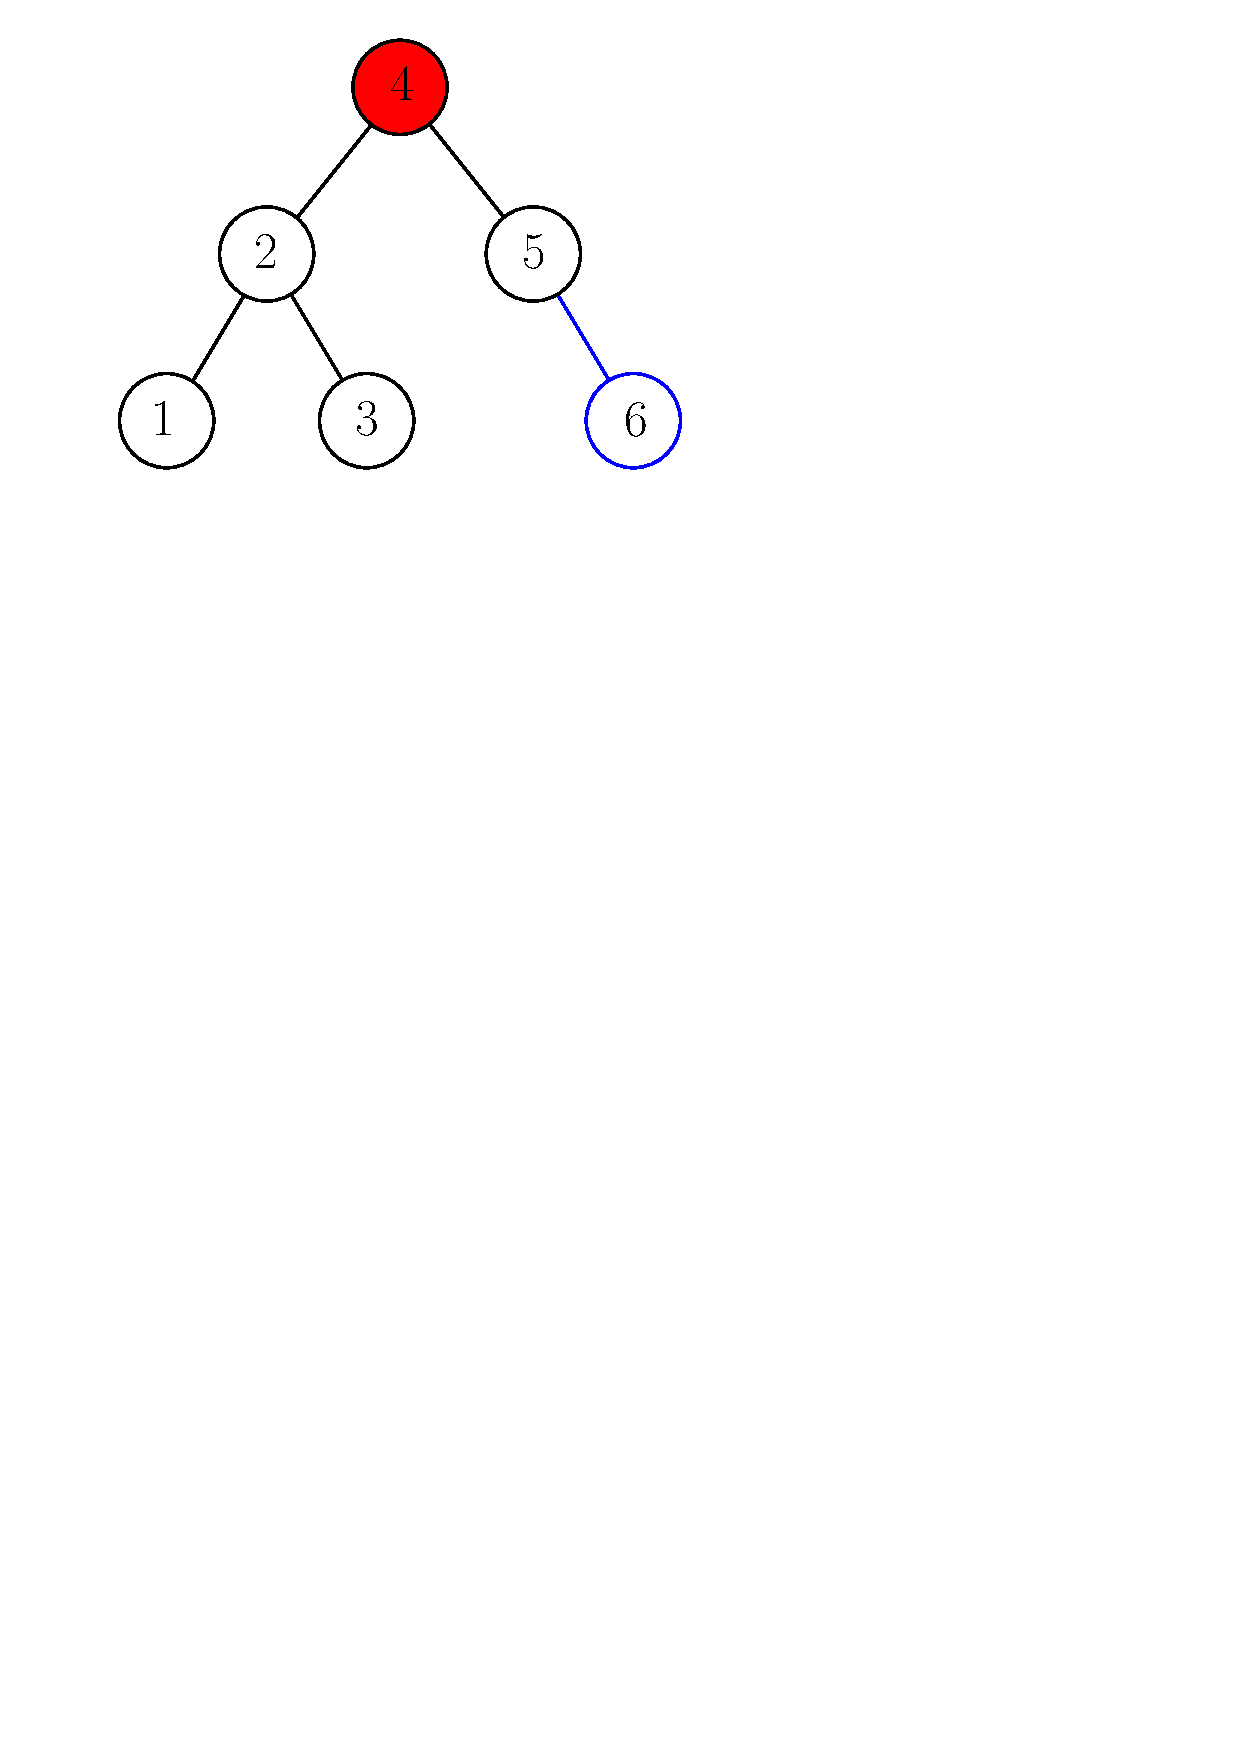
\includegraphics[height=30mm]{./images/binary_searchtree3.pdf}\hfill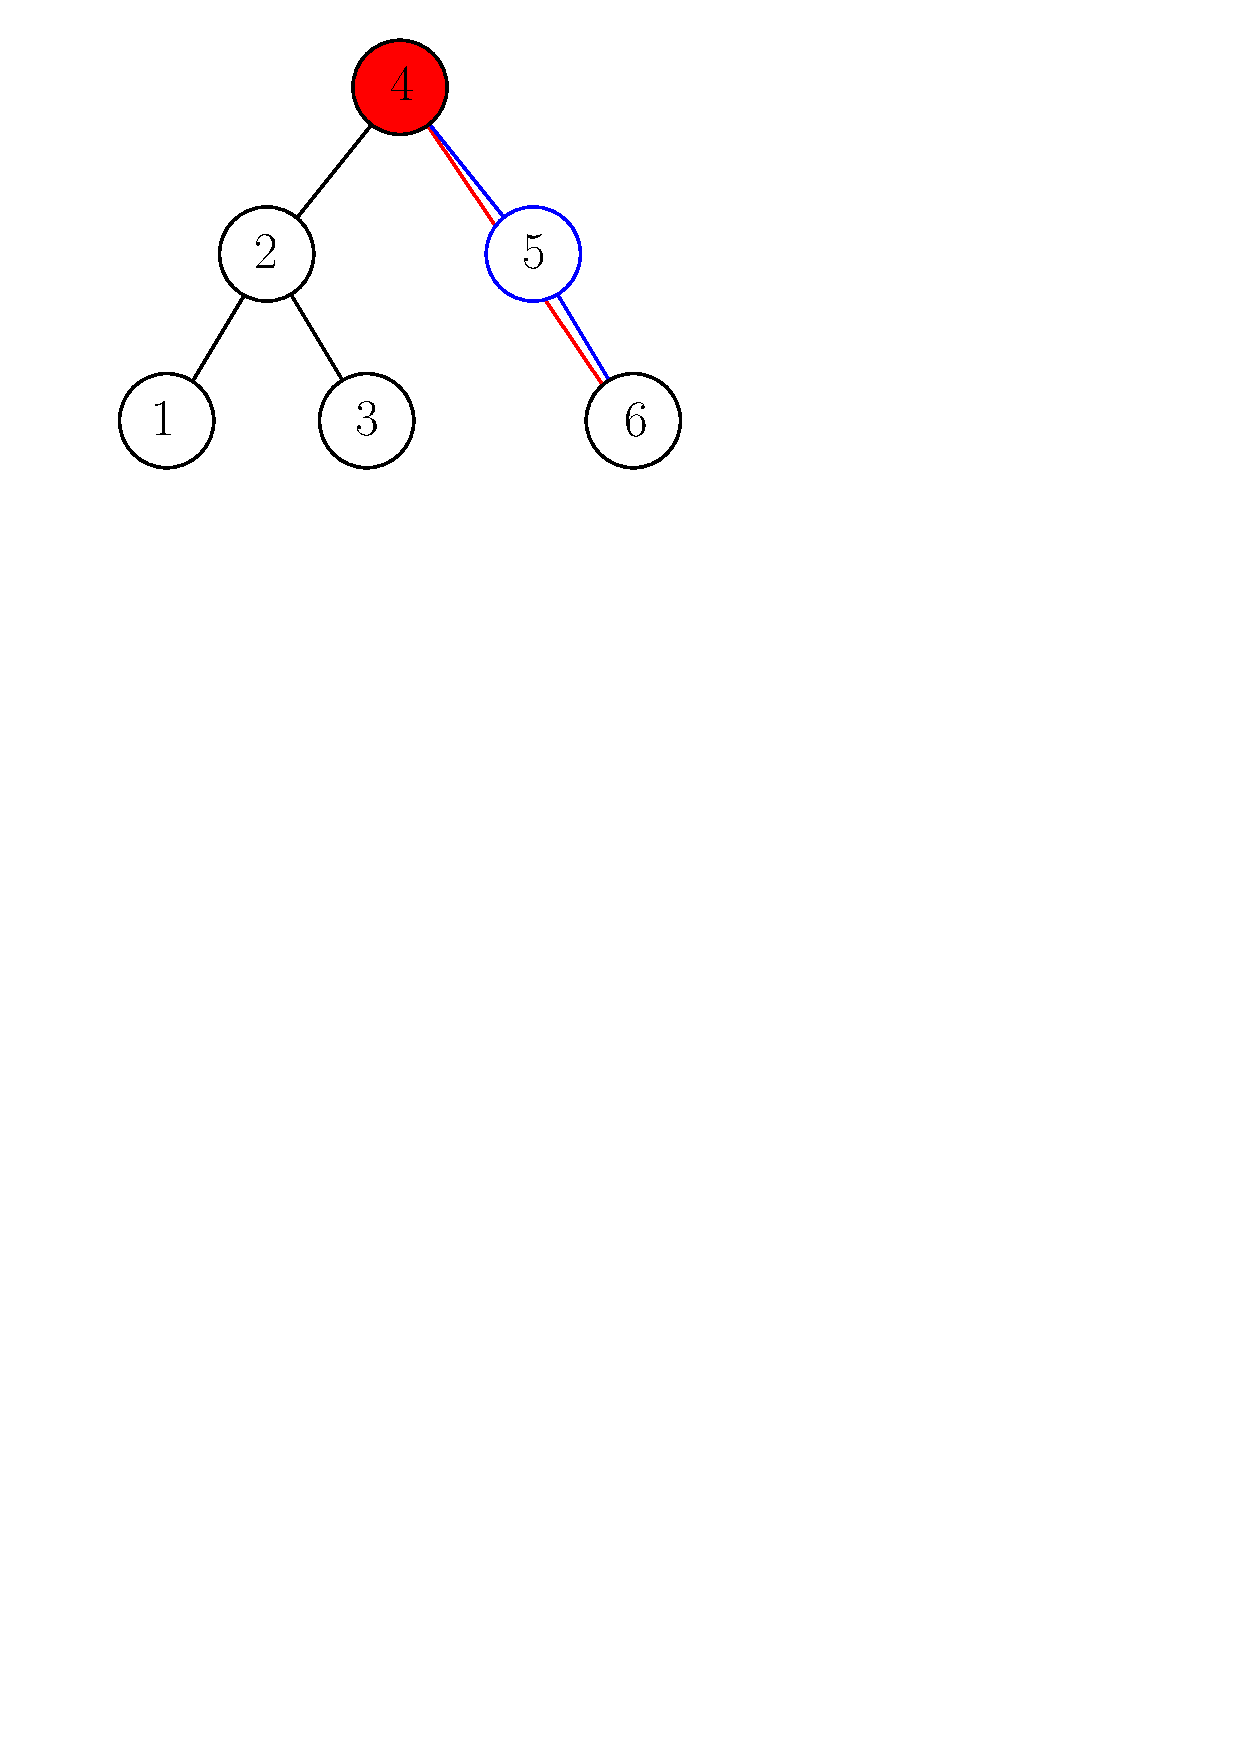
\includegraphics[height=30mm]{./images/binary_searchtree4.pdf}
		\onslide<2>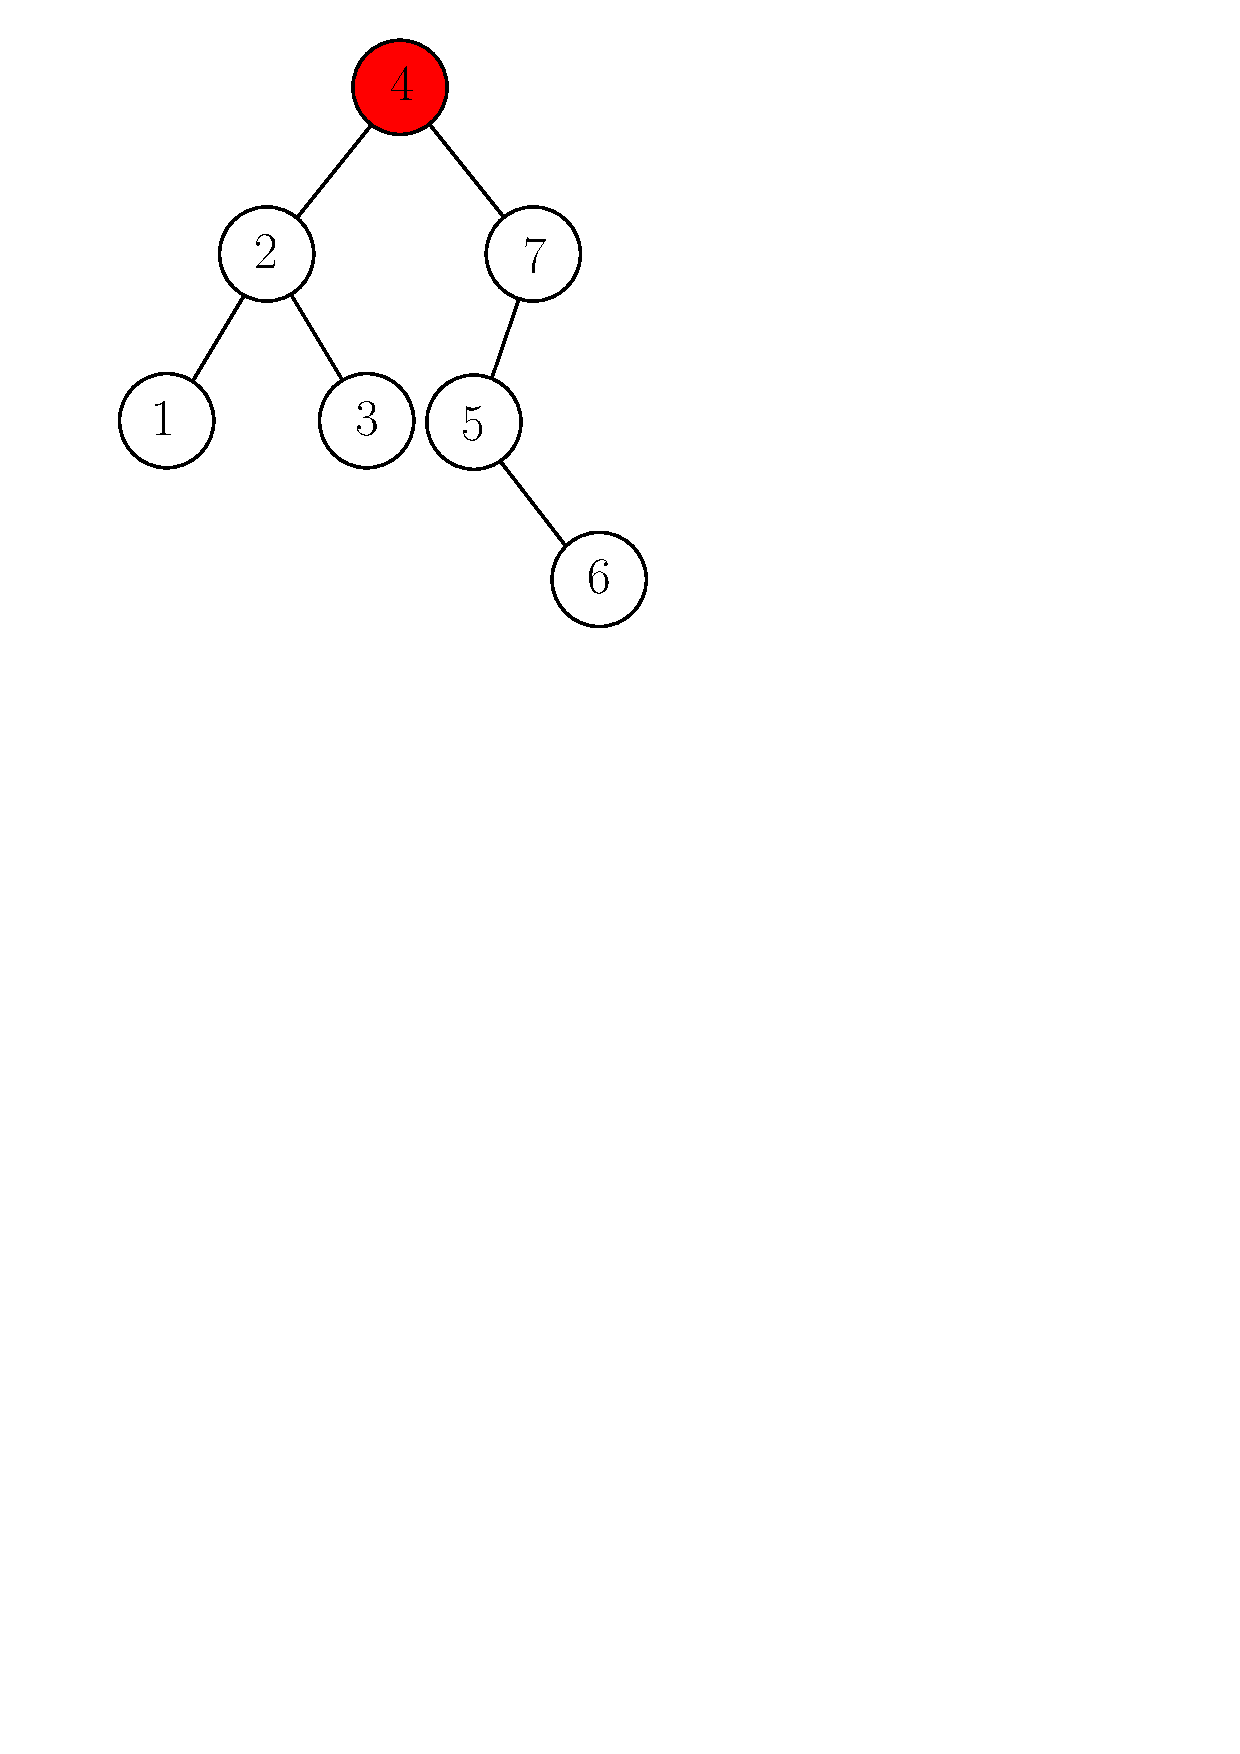
\includegraphics[height=30mm]{./images/binary_searchtree5.pdf}\hfill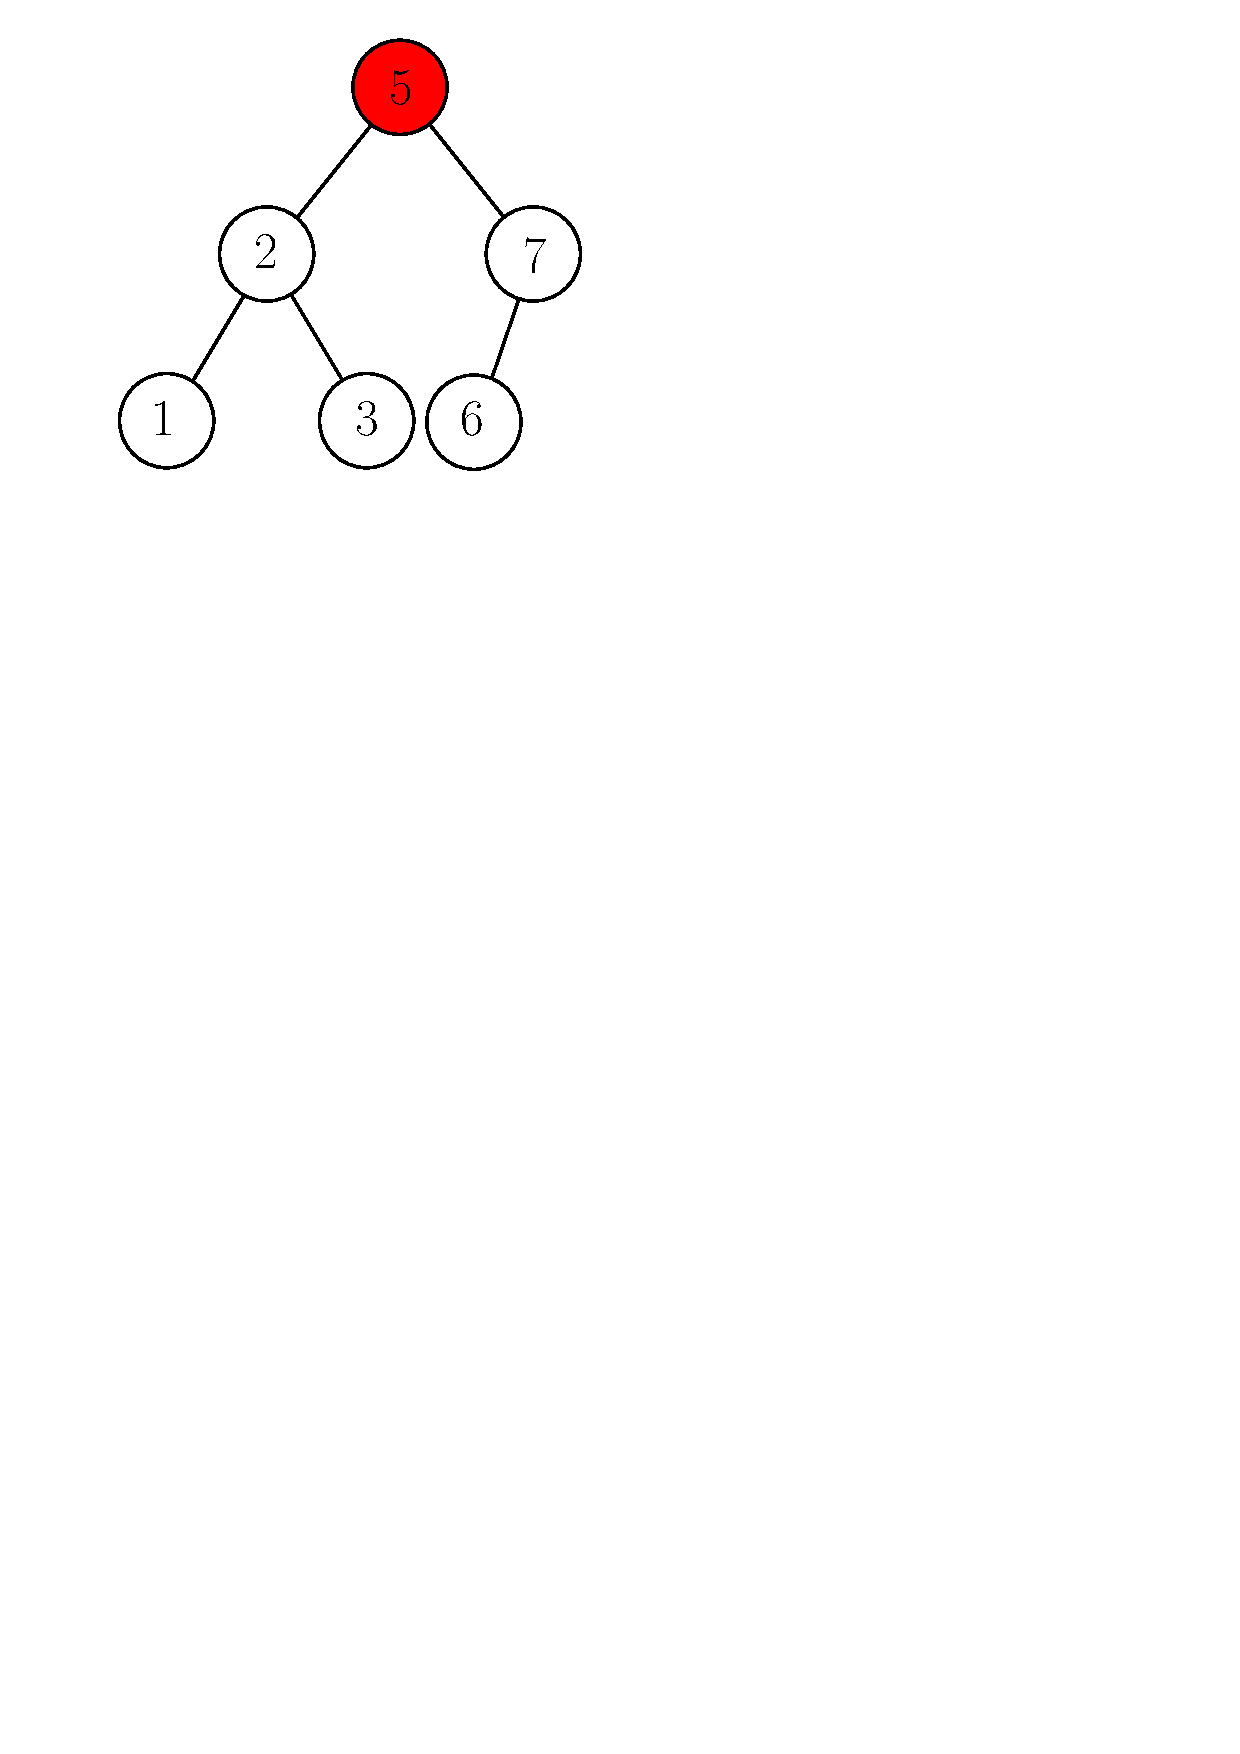
\includegraphics[height=30mm]{./images/binary_searchtree6.pdf}
	\end{overprint}
	\begin{overprint}
		\onslide<1>
		\begin{exampleblock}{Entfernen eines Knotens $v$}
			\begin{itemize}
				\item falls $v$ kein Kind hat, wird $v$ einfach gel\"oscht
				\item falls $v$ nur ein Kind hat, nimmt dieses Kind die Position von $v$ ein
			\end{itemize}
		\end{exampleblock}
		\onslide<2>
		\begin{exampleblock}{Entfernen eines Knotens $v$}
			\begin{itemize}
				\item falls $v$ zwei Kinder hat, finde den Nachfolger $w$ von $z$; $w$ hat nur ein Kind $x$
				\item $w$ nimmt die Stelle von $v$ ein, und $x$ tritt an die Stelle von $w$
			\end{itemize}
		\end{exampleblock}
		\onslide<3>
		\begin{exampleblock}{Laufzeit einf\"ugen/entfernen}
			\begin{itemize}
				\item beide Operationen haben Laufzeit $O(H(t))$
			\end{itemize}
		\end{exampleblock}
	\end{overprint}
\end{frame}

\begin{frame}\frametitle{\mytitle}
		\begin{exampleblock}{Zusammenfassung}
			\begin{itemize}
				\item bin\"are Suchb\"aume erlauben effiziente Operationen, wenn $H(T)$ ``klein'' ist
				\item die optimale H\"ohe bei $n$ Knoten ist $H(T)=O(\log n)$
				\item mit den beschriebenen Operationen kann jedoch der Baum zu einem Pfad ``degenerieren''
				\item dann sind die Operationen nicht effizienter als bei einer verketteten Liste
			\end{itemize}
		\end{exampleblock}
\end{frame}

\end{document}
